\paragraph{Gestione Domande}

\label{Gestione Domande - gestione delle domande create da un utente}

\begin{figure}[ht]
	\centering
	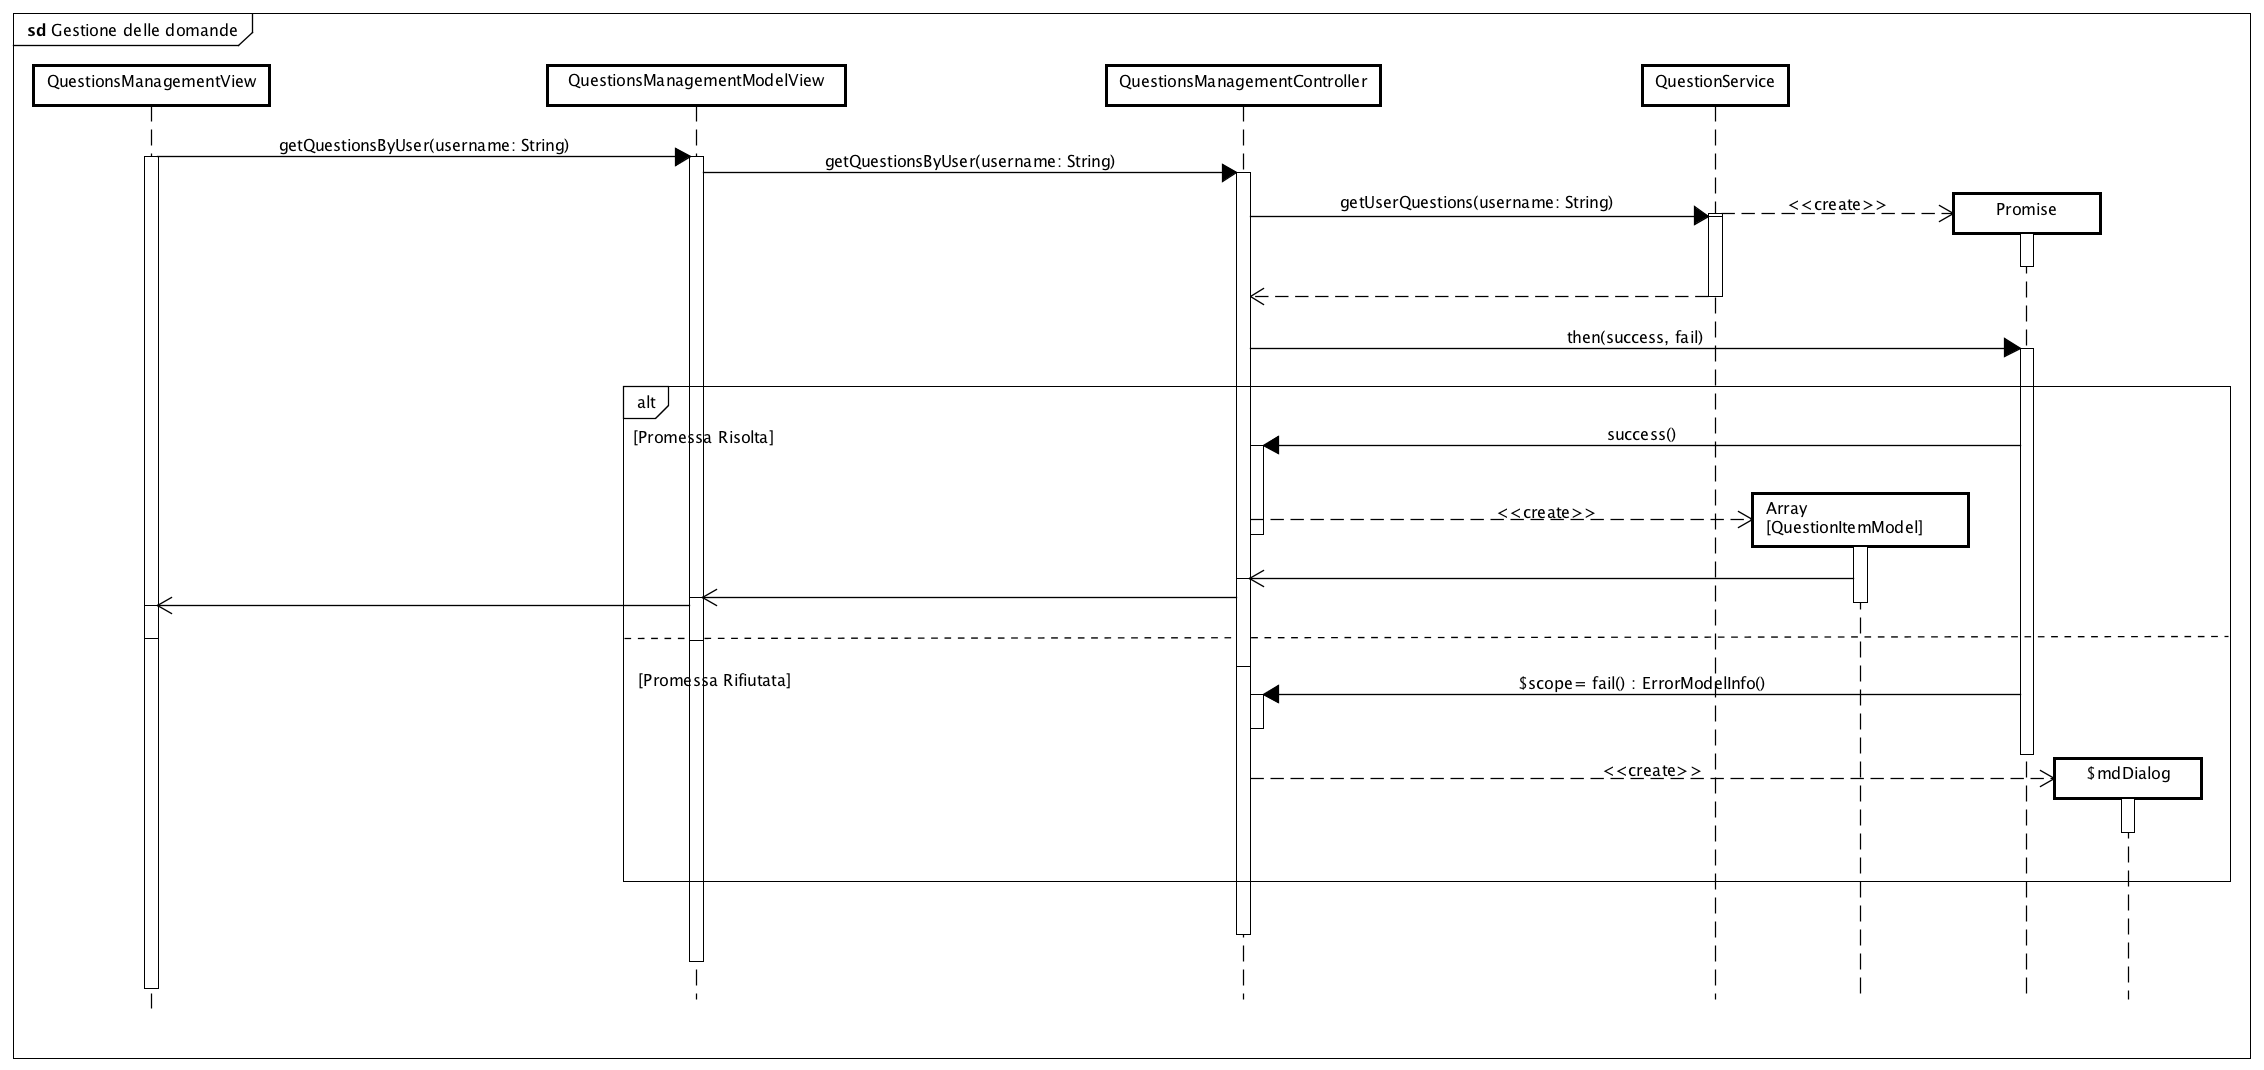
\includegraphics[scale=0.25,keepaspectratio]{UML/DiagrammiDiSequenza/Front-End/QuestionsManagement.png}
	\caption{Gestione Domande - gestione delle domande create da un utente}
\end{figure} \FloatBarrier

Nella view di visualizzazione domande verrà chiamato il metodo del controller che serve per ottenere tutte le domande create dall'utente autenticato. Il controller eseguirà una richiesta al service. A sua volta il service ritornerà una promise che potrà essere risolta o rifiutata. Nel caso venga risolta verrà ritornato l'array di domande ottenuto dal back-end, nel caso invece venga rifiutata verrà restituito un oggetto contenente l'errore e visualizzato un messaggio informativo. 